\paragraph{1.2.2. Share Projection Layer (Tầng chiếu không gian chung)}
\indent\indent Mục tiêu của tầng này là đồng bộ hóa các vector đặc trưng từ ba phương thức khác nhau về cùng một không gian biểu diễn có số chiều cố định (512 chiều), với kiến trúc chi tiết tại \textbf{Hình \ref{fig:KTShareProjectionLayer}}.

\begin{figure}[H]
    \centering
    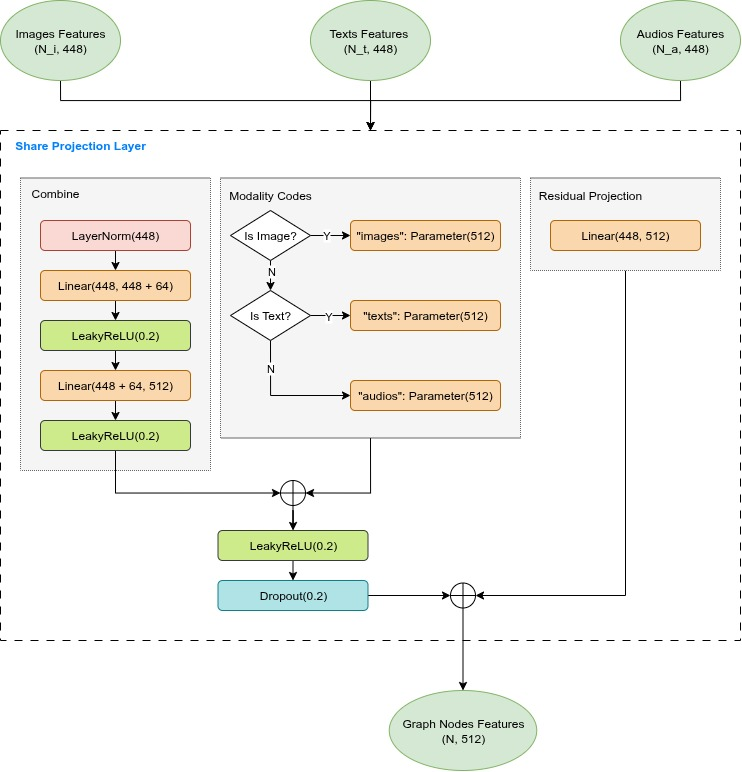
\includegraphics[width=0.8\linewidth]{images/part-02/chap-02/sec-01/ShareProjectionLayer.jpg}
    \vspace{0.3cm}
    \caption{Kiến trúc của Share Projection Layer}
    \label{fig:KTShareProjectionLayer}
\end{figure}

Để phân biệt được phương thức của từng vector đặc trưng trong không gian chung, mô hình sử dụng kỹ thuật Modality Embeddings (hay Modality Codes). Mỗi phương thức được gán một vector tham số học được riêng biệt, cộng trực tiếp vào đặc trưng đầu ra nhằm "đánh dấu" vị trí của nó trong không gian vector chung. Kỹ thuật này được lấy cảm hứng từ cơ chế Token Type Embeddings trong mô hình BERT, giúp mô hình nhận biết ngữ cảnh phương thức \cite{devlin2019bertpretrainingdeepbidirectional}. Đồng thời, cơ chế Residual Connection tiếp tục được áp dụng tại đây nhằm duy trì luồng thông tin xuyên suốt, tránh sự mất mát dữ liệu do các phép biến đổi của tầng Linear.